\documentclass{article}\usepackage[]{graphicx}\usepackage[]{color}
%% maxwidth is the original width if it is less than linewidth
%% otherwise use linewidth (to make sure the graphics do not exceed the margin)
\makeatletter
\def\maxwidth{ %
  \ifdim\Gin@nat@width>\linewidth
    \linewidth
  \else
    \Gin@nat@width
  \fi
}
\makeatother

\definecolor{fgcolor}{rgb}{0.345, 0.345, 0.345}
\newcommand{\hlnum}[1]{\textcolor[rgb]{0.686,0.059,0.569}{#1}}%
\newcommand{\hlstr}[1]{\textcolor[rgb]{0.192,0.494,0.8}{#1}}%
\newcommand{\hlcom}[1]{\textcolor[rgb]{0.678,0.584,0.686}{\textit{#1}}}%
\newcommand{\hlopt}[1]{\textcolor[rgb]{0,0,0}{#1}}%
\newcommand{\hlstd}[1]{\textcolor[rgb]{0.345,0.345,0.345}{#1}}%
\newcommand{\hlkwa}[1]{\textcolor[rgb]{0.161,0.373,0.58}{\textbf{#1}}}%
\newcommand{\hlkwb}[1]{\textcolor[rgb]{0.69,0.353,0.396}{#1}}%
\newcommand{\hlkwc}[1]{\textcolor[rgb]{0.333,0.667,0.333}{#1}}%
\newcommand{\hlkwd}[1]{\textcolor[rgb]{0.737,0.353,0.396}{\textbf{#1}}}%

\usepackage{framed}
\makeatletter
\newenvironment{kframe}{%
 \def\at@end@of@kframe{}%
 \ifinner\ifhmode%
  \def\at@end@of@kframe{\end{minipage}}%
  \begin{minipage}{\columnwidth}%
 \fi\fi%
 \def\FrameCommand##1{\hskip\@totalleftmargin \hskip-\fboxsep
 \colorbox{shadecolor}{##1}\hskip-\fboxsep
     % There is no \\@totalrightmargin, so:
     \hskip-\linewidth \hskip-\@totalleftmargin \hskip\columnwidth}%
 \MakeFramed {\advance\hsize-\width
   \@totalleftmargin\z@ \linewidth\hsize
   \@setminipage}}%
 {\par\unskip\endMakeFramed%
 \at@end@of@kframe}
\makeatother

\definecolor{shadecolor}{rgb}{.97, .97, .97}
\definecolor{messagecolor}{rgb}{0, 0, 0}
\definecolor{warningcolor}{rgb}{1, 0, 1}
\definecolor{errorcolor}{rgb}{1, 0, 0}
\newenvironment{knitrout}{}{} % an empty environment to be redefined in TeX

\usepackage{alltt}
\IfFileExists{upquote.sty}{\usepackage{upquote}}{}
\begin{document}

\title{The socio-cultural sources of urban buzz}
\author{Daniel Arribas-Bel, Karima Kourtit, Peter Nijkamp}
\maketitle
\abstract{Cities have become playing grounds for competitive behaviour and rapid economic dynamics. But in many cities (or urban agglomerations) economic growth is mainly manifested in specific geographic areas, where creative people and innovative entrepreneurs are located. This paper offers first the foundation for analysing the so-called 'urban buzz' and its interlinked primary drivers. The paper will next develop an analytical framework for testing the buzz hypothesis, with a special reference to the importance of social networks in Amsterdam. In our empirical analysis, we use a unique data set on social network connectivity and spatial concentration in a city, based on location-sharing services through the use of Foursquare. Our urban buzz model shows clearly that buzz and socio-economic (cultural) diversity are closely connected phenomena.}

\section{Reading the data}

First, we read in some stuff and do some simple descriptives (we do no display them here)

\begin{knitrout}
\definecolor{shadecolor}{rgb}{0.969, 0.969, 0.969}\color{fgcolor}\begin{kframe}
\begin{alltt}
\hlstd{db} \hlkwb{<-} \hlkwd{read.csv}\hlstd{(}\hlstr{"~/Thomas/Colleges/WooW/examples/buzz_data.csv"}\hlstd{)}
\hlkwd{head}\hlstd{(db)}
\hlkwd{tail}\hlstd{(db)}
\hlkwd{summary}\hlstd{(db)}
\hlkwd{library}\hlstd{(stargazer)}
\end{alltt}


{\ttfamily\noindent\itshape\color{messagecolor}{\#\# \\\#\# Please cite as: \\\#\# \\\#\#\ \ Hlavac, Marek (2013). stargazer: LaTeX code and ASCII text for well-formatted regression and summary statistics tables.\\\#\#\ \ R package version 4.5.3. http://CRAN.R-project.org/package=stargazer}}\end{kframe}
\end{knitrout}

Then we are interested in some nice plots
\begin{knitrout}
\definecolor{shadecolor}{rgb}{0.969, 0.969, 0.969}\color{fgcolor}\begin{kframe}
\begin{alltt}
\hlkwd{plot}\hlstd{(}\hlkwd{density}\hlstd{(db}\hlopt{$}\hlstd{div_i))}
\end{alltt}
\end{kframe}
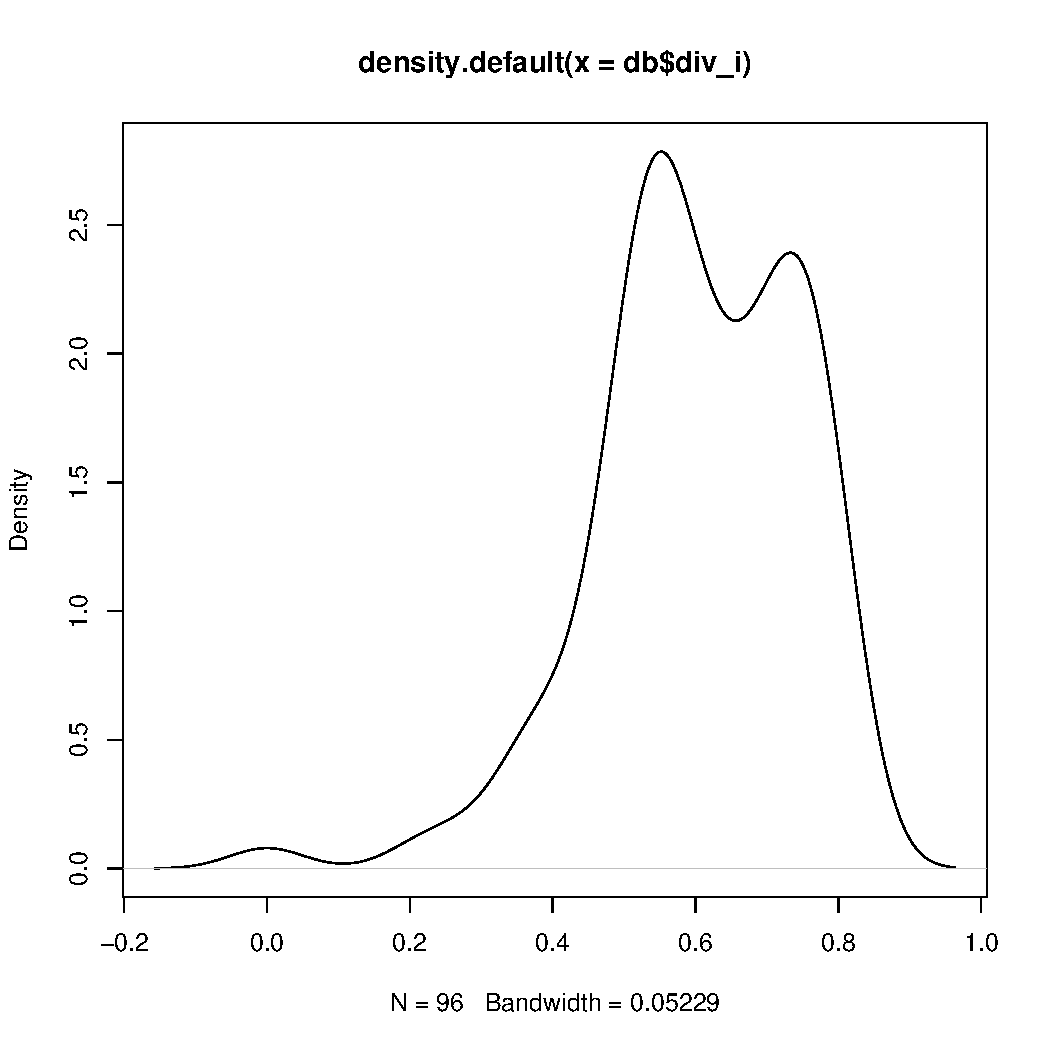
\includegraphics[width=\maxwidth]{figure/foo1} 

\end{knitrout}


\begin{knitrout}
\definecolor{shadecolor}{rgb}{0.969, 0.969, 0.969}\color{fgcolor}\begin{kframe}
\begin{alltt}
\hlkwd{plot}\hlstd{(db}\hlopt{$}\hlstd{div_i, db}\hlopt{$}\hlstd{industrie_pct_area)}
\end{alltt}
\end{kframe}
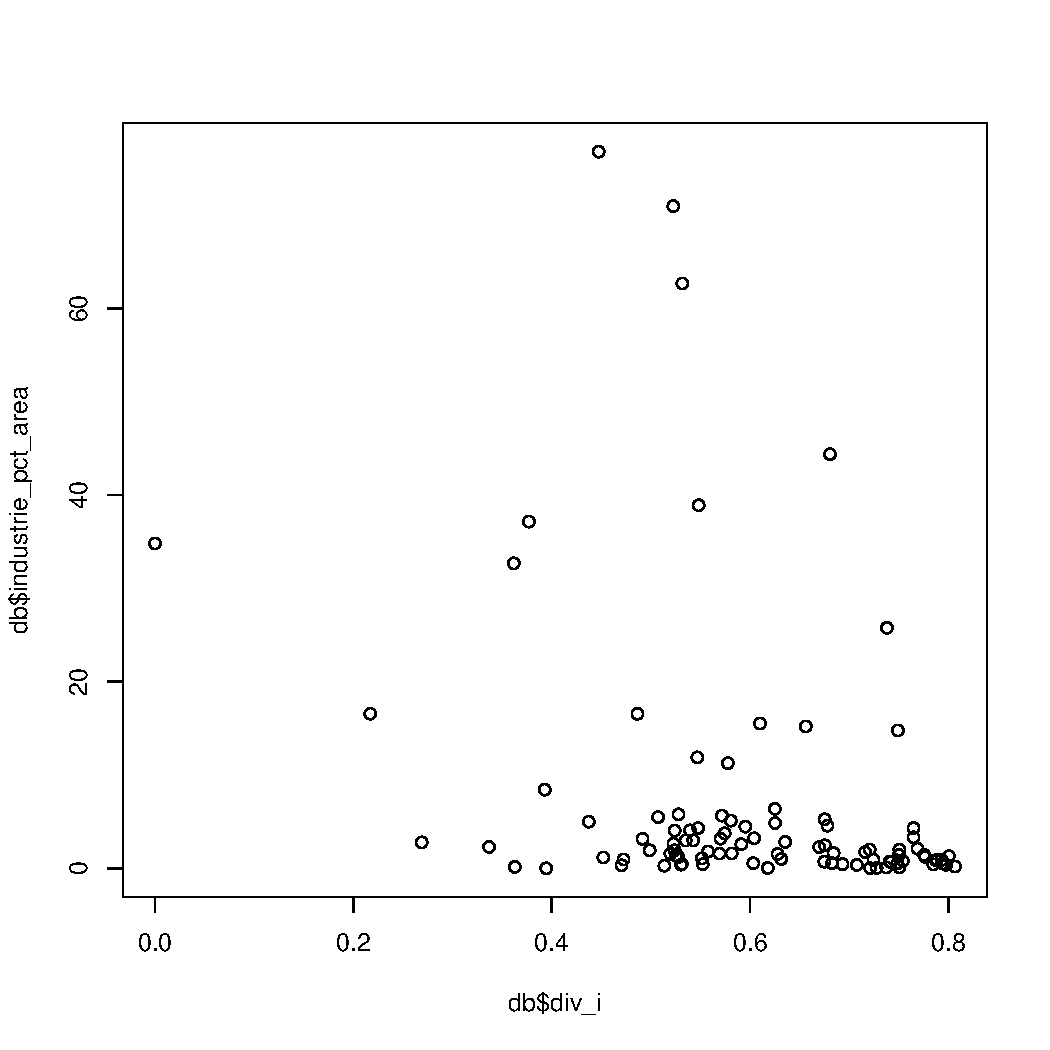
\includegraphics[width=\maxwidth]{figure/foo5} 

\end{knitrout}

And finally we do a simple OLS and display the results in a {\LaTeX} table
\begin{knitrout}
\definecolor{shadecolor}{rgb}{0.969, 0.969, 0.969}\color{fgcolor}\begin{kframe}
\begin{alltt}
\hlstd{ols} \hlkwb{<-} \hlkwd{lm}\hlstd{(checkins_all} \hlopt{~} \hlstd{total_units} \hlopt{+} \hlstd{div_i,} \hlkwc{data} \hlstd{= db)}
\end{alltt}
\end{kframe}
\end{knitrout}




% Table created by stargazer v.4.5.3 by Marek Hlavac, Harvard University. E-mail: hlavac at fas.harvard.edu
% Date and time: Thu, Jan 16, 2014 - 09:35:00
\begin{table}[!htbp] \centering 
  \caption{Regression results} 
  \label{} 
\begin{tabular}{@{\extracolsep{5pt}}lc} 
\\[-1.8ex]\hline 
\hline \\[-1.8ex] 
\\[-1.8ex] & checkins\_all \\ 
\hline \\[-1.8ex] 
 total\_units & 0.114$^{***}$ \\ 
  & (0.039) \\ 
  & \\ 
 div\_i & $-$1,101.000 \\ 
  & (814.700) \\ 
  & \\ 
 Constant & 918.600$^{**}$ \\ 
  & (454.600) \\ 
  & \\ 
Observations & 96 \\ 
R$^{2}$ & 0.083 \\ 
Adjusted R$^{2}$ & 0.063 \\ 
Residual Std. Error & 1,036.000 (df = 93) \\ 
F Statistic & 4.219$^{**}$ (df = 2; 93) \\ 
\hline \\[-1.8ex] 
\textit{Notes:} & \multicolumn{1}{l}{$^{***}$Significant at the 1 percent level.} \\ 
 & \multicolumn{1}{l}{$^{**}$Significant at the 5 percent level.} \\ 
 & \multicolumn{1}{l}{$^{*}$Significant at the 10 percent level.} \\ 
\normalsize 
\end{tabular} 
\end{table} 



\end{document}
